\documentclass[aspectratio=169,10pt]{beamer}

\usetheme[progressbar=frametitle]{metropolis}
\usepackage{appendixnumberbeamer}
\usepackage{tikz}
\usetikzlibrary{positioning}
\usepackage{booktabs}
\usepackage[scale=2]{ccicons}

\usepackage{pgfplots}
\usepgfplotslibrary{dateplot}

\usepackage{xspace}
\newcommand{\themename}{\textbf{\textsc{metropolis}}\xspace}

\usepackage[spanish,es-tabla]{babel}

\usepackage{xcolor}
\definecolor{dkgreen}{rgb}{0,0.6,0}
\definecolor{gray}{rgb}{0.5,0.5,0.5}
\definecolor{mauve}{rgb}{0.58,0,0.82}
\usepackage{listings}
\lstset{%
	numberstyle=\tiny,
	basicstyle=\fontsize{6.5}{8.3}\ttfamily,
	numbersep=15pt,tabsize=4,
	flexiblecolumns=true,
	keywordstyle=\color{blue},
	commentstyle=\color{dkgreen},
	stringstyle=\color{mauve},
	numberstyle=\tiny\color{gray},
	language=Java,
	breaklines=true,
	breakatwhitespace=true,
  showstringspaces=false,
  aboveskip=0.1em,
  belowskip=0.5em,
	morekeywords={*,num,String,var,library,get,set,StringEq,StringHashEq,bool,Top,Bot,<,String@L,String@H,int@L,int@H,bool@H,bool@L} ,
}


\title{DESCLASIFICACIÓN BASADA EN TIPOS EN DART}
\subtitle{IMPLEMENTACIÓN Y ELABORACIÓN DE HERRAMIENTAS DE INFERENCIA}
% \date{\today}
\date{}
\author{Matías Meneses Cortés}
%\institute{Departamento de Ciencias de la Computación}
\titlegraphic{\hfill
\includegraphics[height=2.5cm]{logo.png}}

\begin{document}

\maketitle

\begin{frame}{Contenidos}
  \setbeamertemplate{section in toc}[sections numbered]
  \tableofcontents[hideallsubsections]
\end{frame}

\section{Control de flujo de información}

\begin{frame}[fragile]{Protección de confidencialidad}
  \begin{center}
    \only<1>{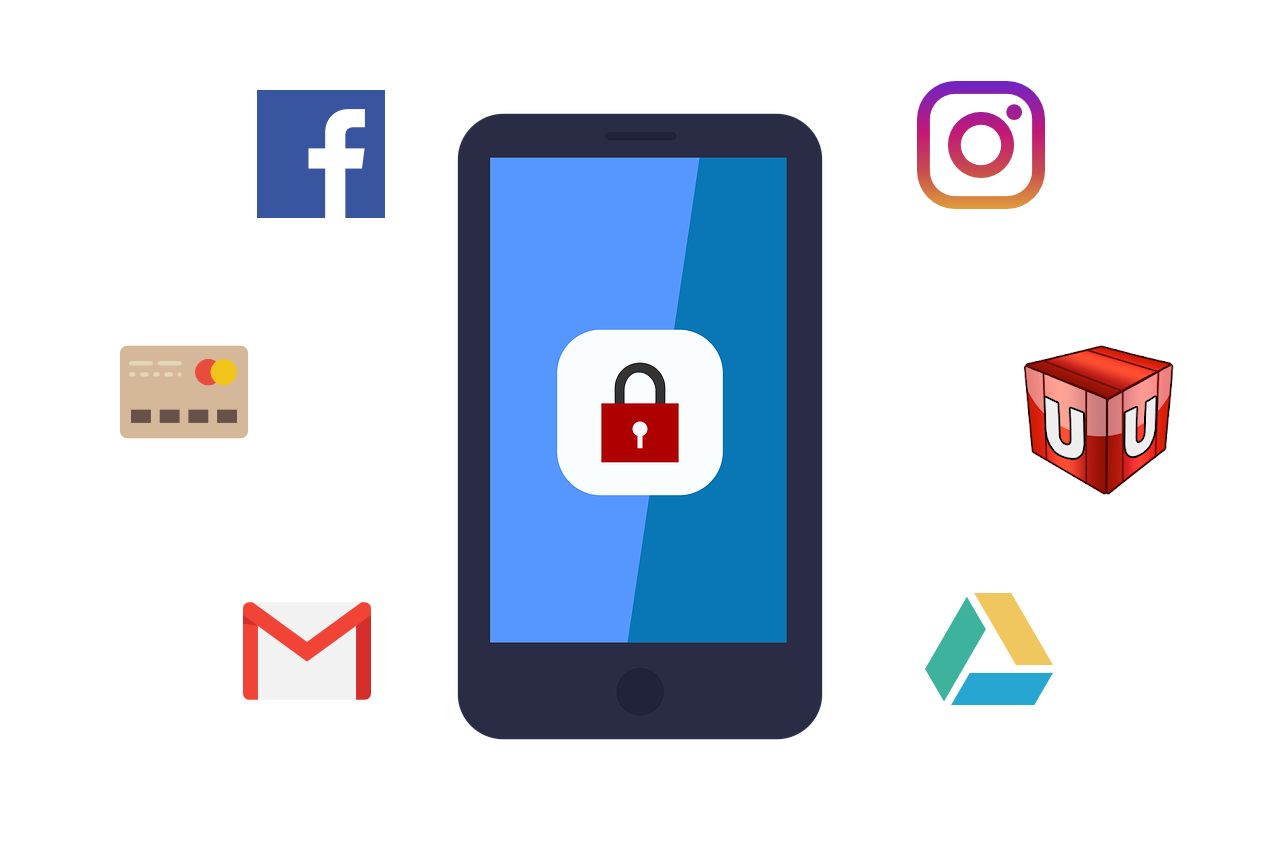
\includegraphics[width=0.8\textwidth]{images/interaccion.png}}
		\only<2>{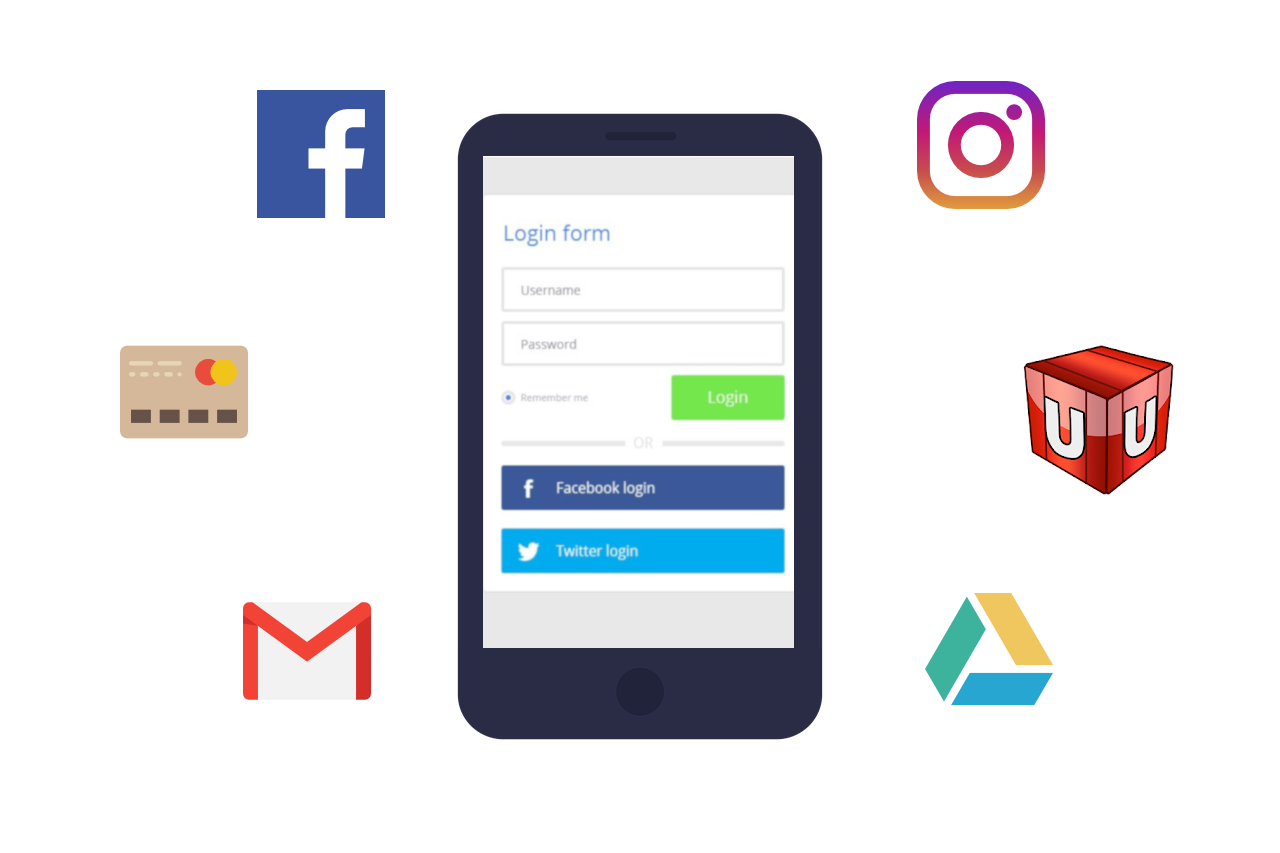
\includegraphics[width=0.8\textwidth]{images/auth.png}}
		\only<3>{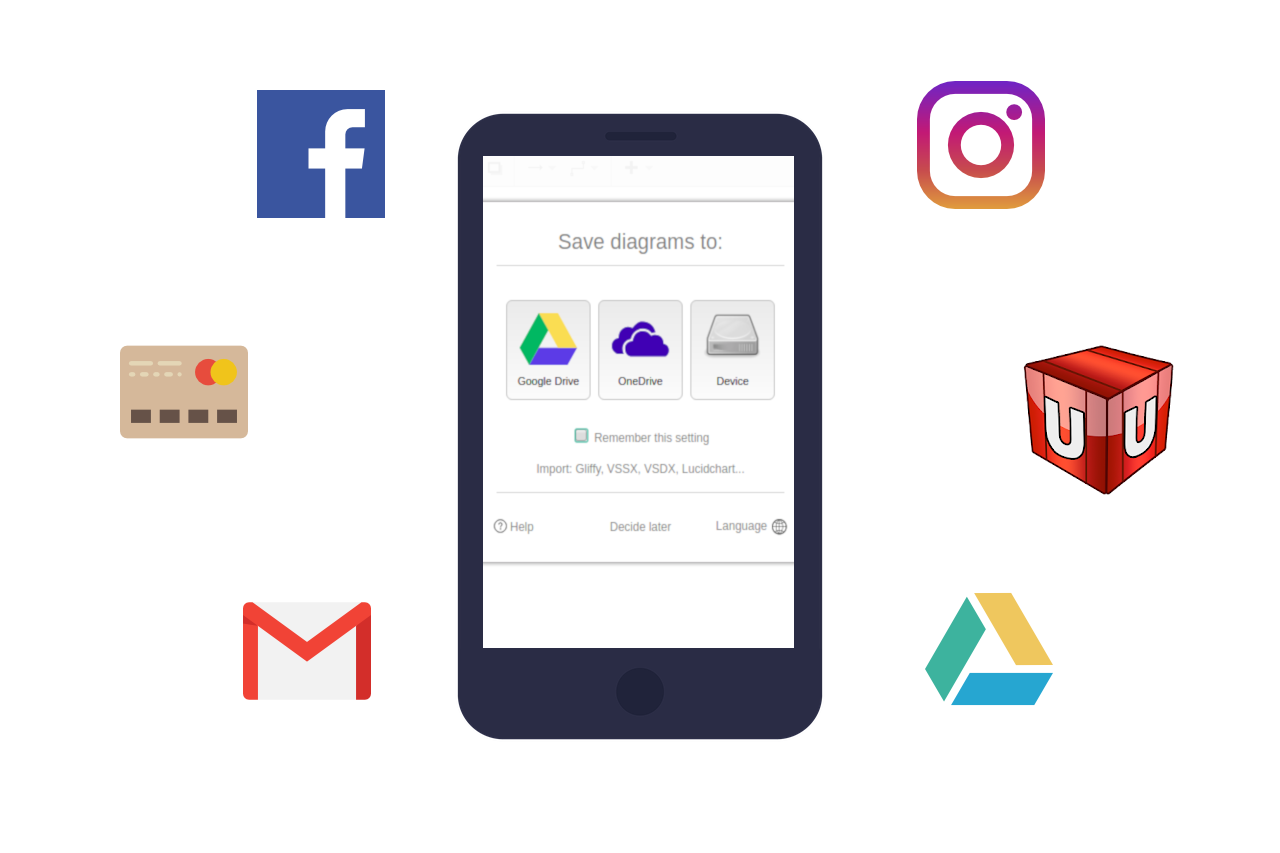
\includegraphics[width=0.8\textwidth]{images/gdrive.png}}
		\only<4>{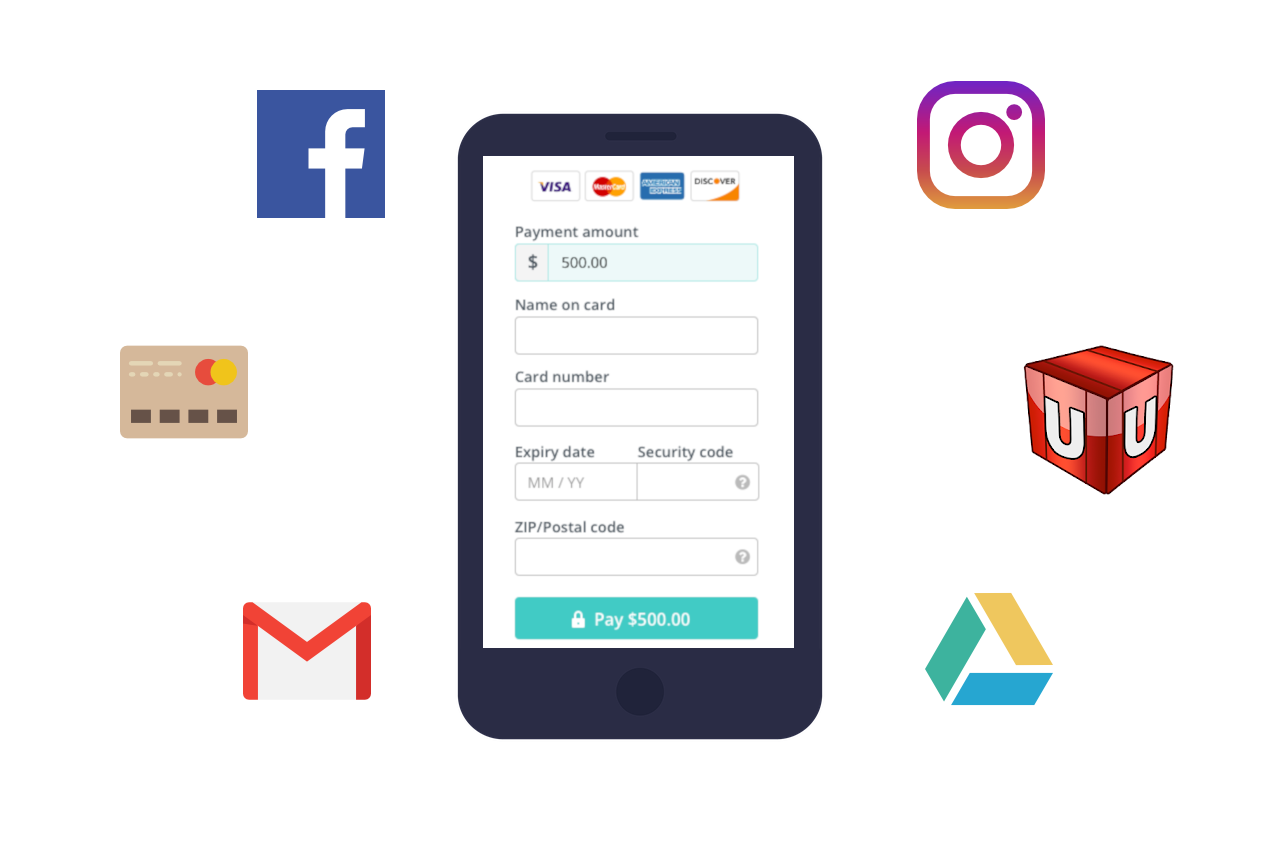
\includegraphics[width=0.8\textwidth]{images/pay.png}}
    \only<5>{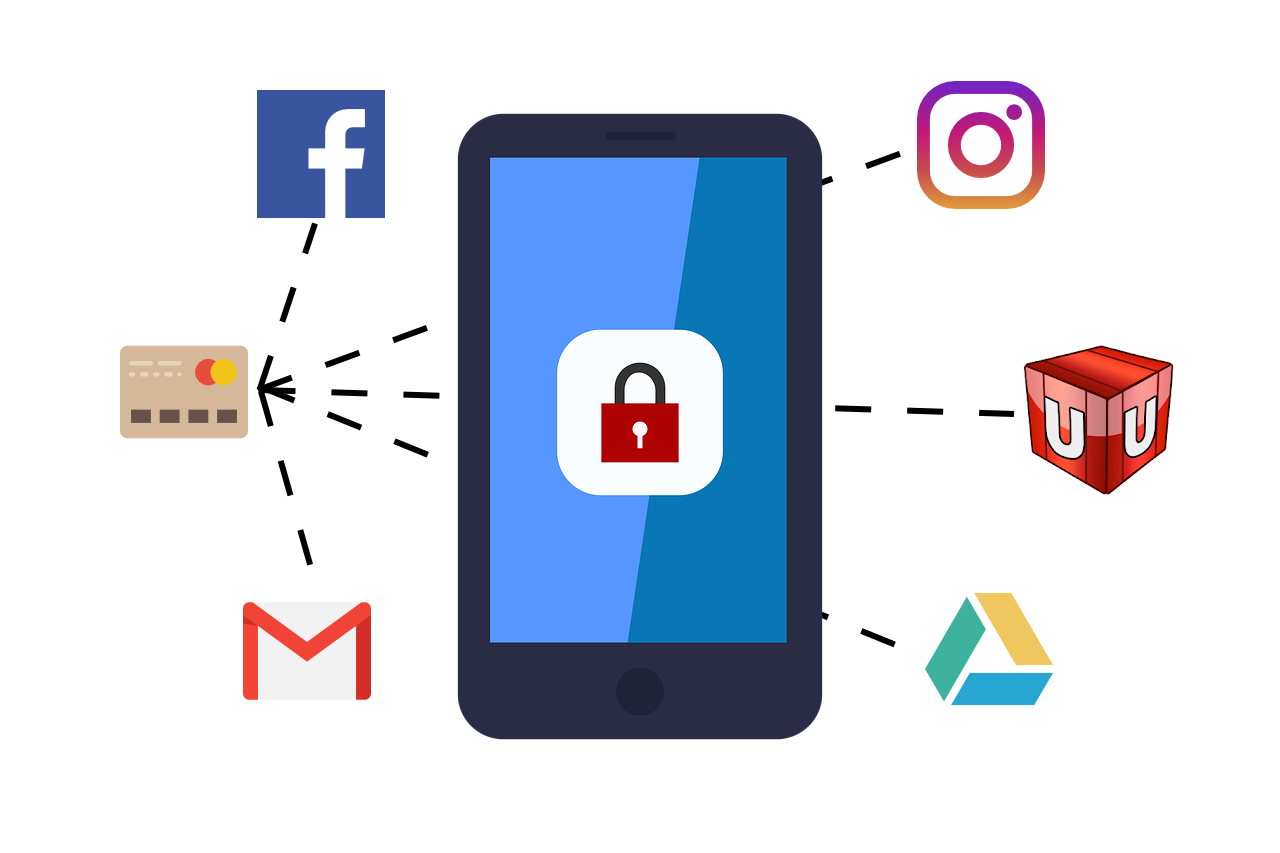
\includegraphics[width=0.8\textwidth]{images/interaccion2.png}}
  \end{center}
\end{frame}

\begin{frame}[fragile]{Protección de confidencialidad}
  Distintas técnicas de seguridad en distintas capas de comunicación. \pause
  \vspace{0.5cm}
  \begin{columns}[T,onlytextwidth]
    \column{0.6\textwidth}
    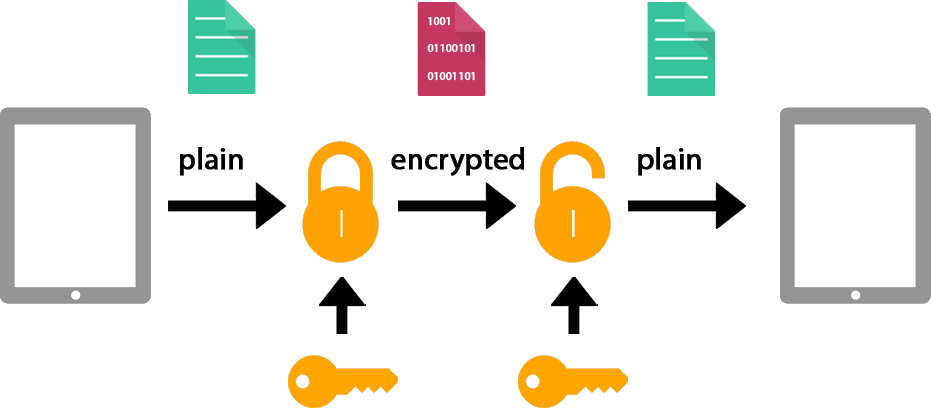
\includegraphics[width=0.8\textwidth]{images/e2e.png} \pause
    \column{0.4\textwidth}
    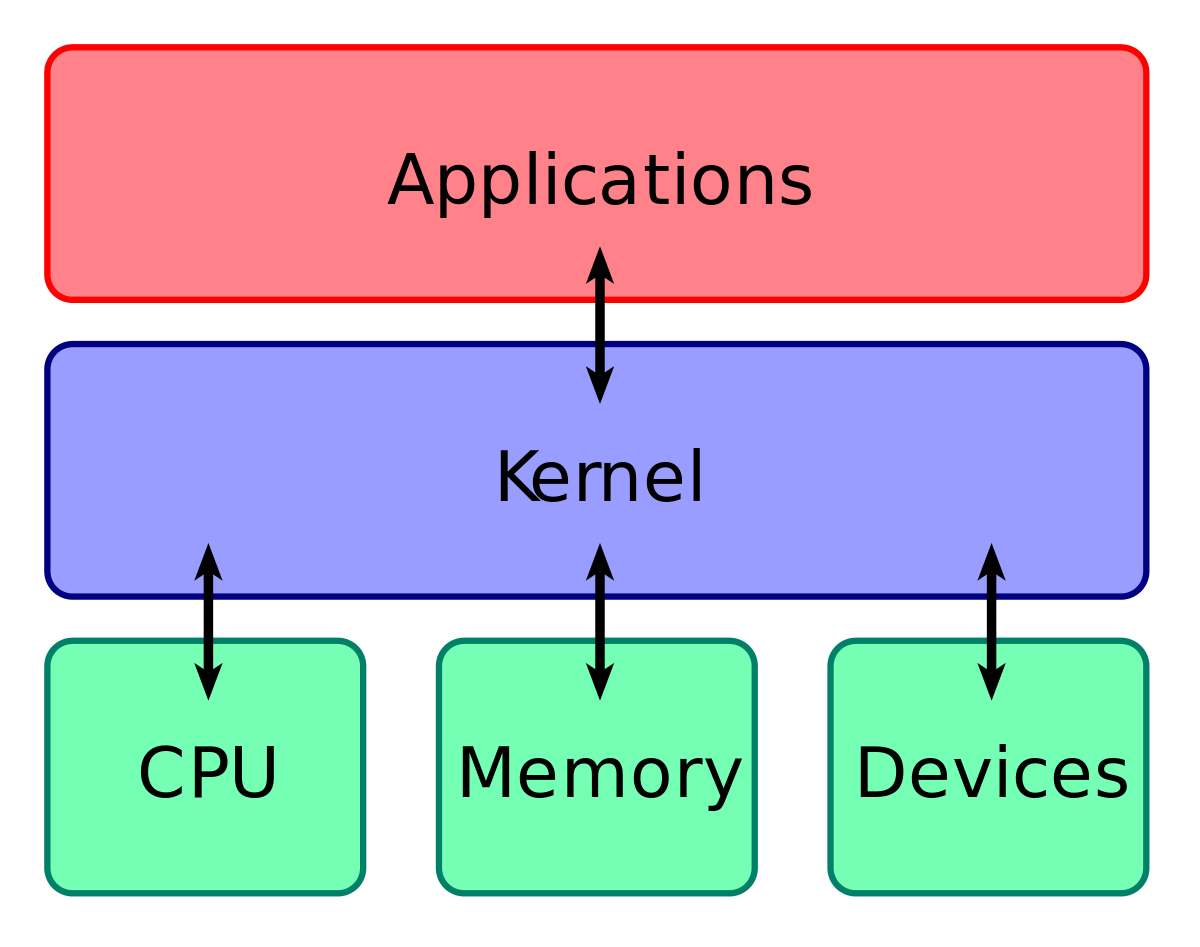
\includegraphics[width=1.0\textwidth]{images/kernel.png}
  \end{columns}
\end{frame}

\begin{frame}[fragile]{Seguridad basada en el lenguaje: Tipado de seguridad}
	\begin{columns}[T,onlytextwidth]
		\column{0.5\textwidth}
		
\includegraphics[width=0.8\textwidth]{images/lbs.png}
		\column{0.5\textwidth}
		\begin{lstlisting}[basicstyle=\fontsize{6.3}{8}\ttfamily]
String@L login(String@L guess, String@H password) {
  if (password == guess) return "Login successful";
  else return "Login failed";
}
    \end{lstlisting}
		\begin{center}
			\begin{tikzpicture}
				\node(H) 												{\texttt{H}};
				\node(L)      [below of=H]       {\texttt{L}};
				\draw(H)      -- (L);
			\end{tikzpicture} \\
			Orden parcial de dos niveles
		\end{center}
	\end{columns}
\end{frame}

\begin{frame}[fragile]{Control de flujo de información}
  \begin{columns}[T,onlytextwidth]
    \column{0.25\textwidth}
    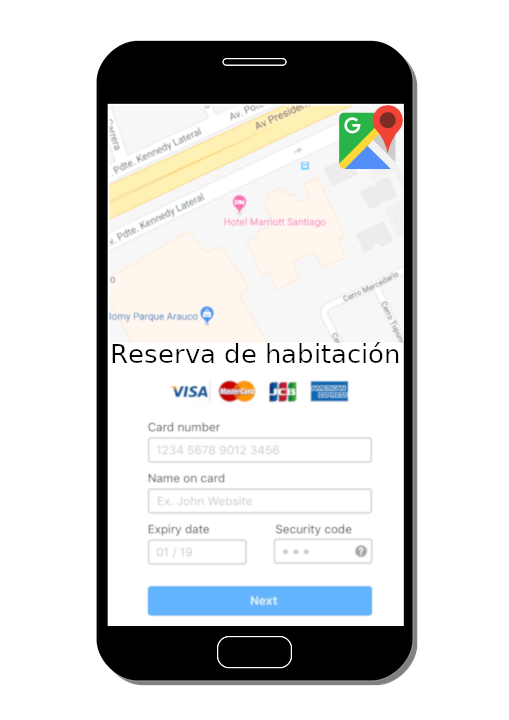
\includegraphics[width=1.0\textwidth]{images/book.png}
    \column{0.75\textwidth}
    \vspace{1cm}
    \begin{onlyenv}<1>
      \begin{lstlisting}
        String book(String username, int date, int cardNumber) {
          return sendToHotel(username, date, cardNumber);
        }

        String sendToHotel(String username, int date, int cardNumber);
        String sendToGoogle(String token, int xCoord, int yCoord);
      \end{lstlisting}
    \end{onlyenv}
    \begin{onlyenv}<2>
      \begin{lstlisting}[escapechar=?]
        String book(String username, int date, int cardNumber) {
          return ?\colorbox{yellow!50}{sendToGoogle}?(username, date, cardNumber);
        }

        String sendToHotel(String username, int date, int cardNumber);
        String sendToGoogle(String token, int xCoord, int yCoord);
      \end{lstlisting}
    \end{onlyenv}

  \end{columns}
\end{frame}

\begin{frame}[fragile]{Tipado de seguridad para el control de flujo de información}

  \begin{columns}[T,onlytextwidth]
    \column{0.25\textwidth}
    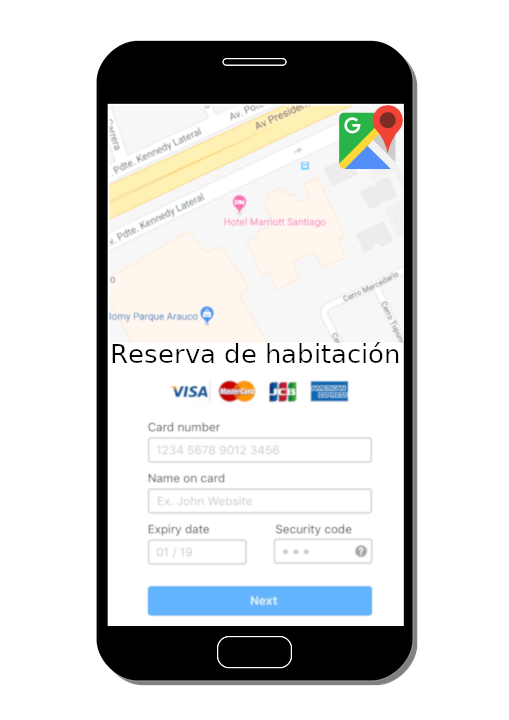
\includegraphics[width=1.0\textwidth]{images/book.png}
    \column{0.75\textwidth}
    \vspace{1cm}
    \begin{onlyenv}<1>
      \begin{lstlisting}
        String@L book(String@L username, int@L date, int@H cardNumber) {
          return sendToGoogle(username, date, cardNumber);
        }

        String@L sendToHotel(String@L username, int@L date, int@H cardNumber);
        String@L sendToGoogle(String@H token, int@L xCoord, int@L yCoord);
      \end{lstlisting}
    \end{onlyenv}
    \begin{onlyenv}<2>
      \begin{lstlisting}[escapechar=?]
        String@L book(String@L username, int@L date, int@H cardNumber) {
          ?\colorbox{red!20}{return sendToGoogle(username, date, cardNumber);}?
        }

        String@L sendToHotel(String@L username, int@L date, int@H cardNumber);
        String@L sendToGoogle(String@H token, int@L xCoord, int@L yCoord);
      \end{lstlisting}
    \end{onlyenv}
		\begin{onlyenv}<3>
      \begin{lstlisting}[escapechar=?]
        String@L book(String@L username, int@L date, int@H cardNumber) {
          return sendToHotel(username, date, cardNumber);
        }

        String@L sendToHotel(String@L username, int@L date, int@H cardNumber);
        String@L sendToGoogle(String@H token, int@L xCoord, int@L yCoord);
      \end{lstlisting}
    \end{onlyenv}
  \end{columns}

\end{frame}

\begin{frame}[fragile]{No-interferencia}
  Propiedad fundamental del control de flujo de información.
	\begin{center}
		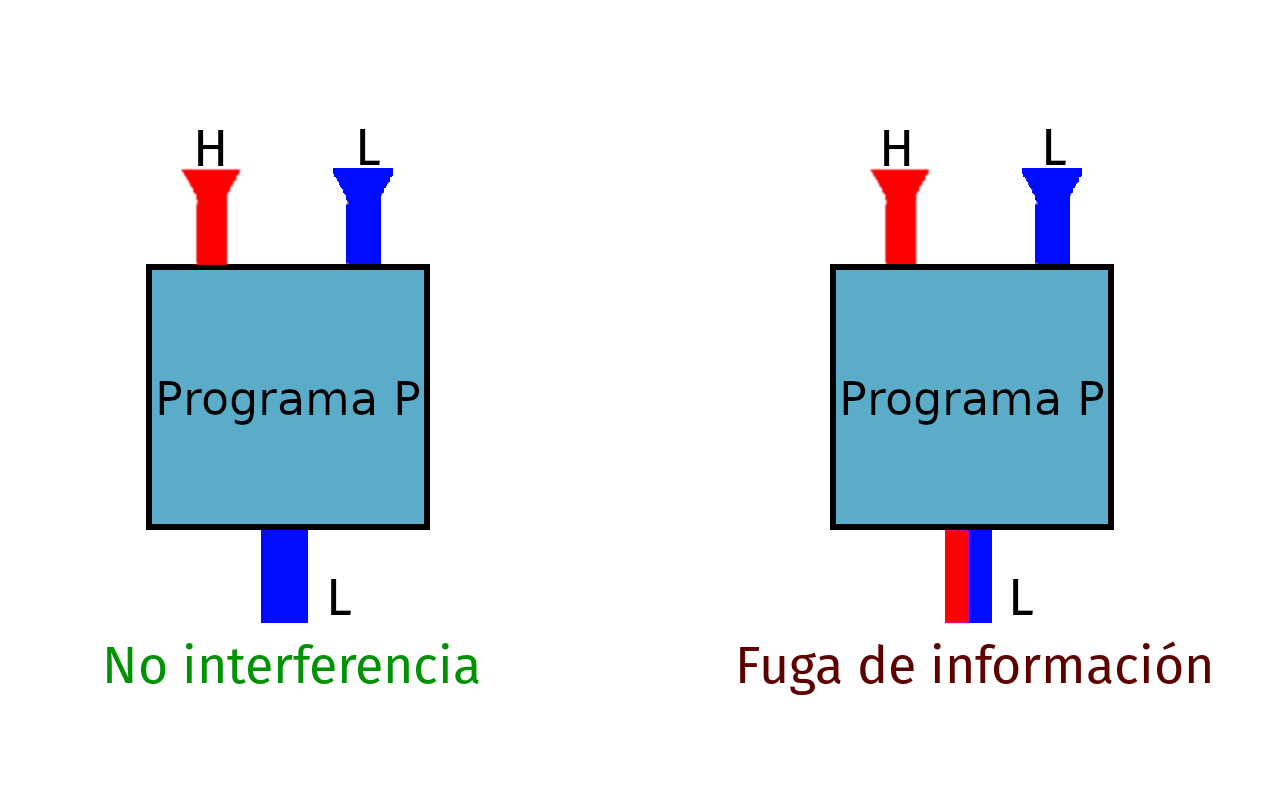
\includegraphics[width=0.8\textwidth]{images/noninterference.png}
	\end{center}
\end{frame}

\begin{frame}[fragile]{Problema con no-interferencia}
	\begin{center}
\begin{lstlisting}[basicstyle=\fontsize{9}{9}\ttfamily]
            String@L login(String@L guess, String@H password) {
              if (password == guess) return "Login successful";
              else return "Login failed";
            }
\end{lstlisting}
		\vspace{3cm}
		\alert{¡\textbf{No} cumple con no-interferencia!}
	\end{center}
\end{frame}

\begin{frame}[fragile]{Desclasificación}
	\begin{center}
\begin{lstlisting}[basicstyle=\fontsize{9}{9}\ttfamily]
            String@L login(String@L guess, String@H password) {
              if (declassify(password == guess)) return "Login successful";
              else return "Login failed";
            }
\end{lstlisting}
	\end{center}
\end{frame}

\begin{frame}[fragile]{Problema con desclasificación}
	\begin{center}
\begin{lstlisting}[basicstyle=\fontsize{9}{9}\ttfamily]
                                    declassify(password)
\end{lstlisting} \pause
		\vspace{3cm}
		\alert{¡Grave fuga de información!}
	\end{center}
\end{frame}

\begin{frame}[fragile]{Desclasificación basada en tipos}
\begin{lstlisting}[basicstyle=\fontsize{9}{9}\ttfamily]
String<String login(String<String guess, String<StringEq password) {
  if (password.eq(guess)) return "Login successful";
  else return "Login failed";
}
\end{lstlisting} \pause

\begin{itemize}
	\item Tipos de dos facetas \texttt{String<StringEq} \pause
	\item \texttt{StringEq = [eq: String<String -> Bool<Bool]} \pause
	\item \texttt{String <: StringEq} (Tipo bien formado) \pause
	\item No-interferencia relajada
\end{itemize}

\end{frame}

\begin{frame}[fragile]{Retículo de subtipos}
	\begin{center}
		\begin{tikzpicture}[node distance=2.1cm]
			\node(Top) 												{\texttt{Top} $\triangleq [\ ]$};
			\node(StringEq)		[below right=0.7cm and 0.1cm of Top]			{\texttt{StringEq} $\triangleq [\mathtt{eq} : \mathtt{String} \rightarrow \mathtt{Bool}]$};
			\node(StringEqLength)      [below of=StringEq]       {\texttt{StringEqLength} $\triangleq [...,\ \mathtt{length: Unit\rightarrow Int]}$};
			\node(String)				[below of=StringEqLength]       {\texttt{String} $\triangleq [...]$};
			\node(int)					[below left=0.7cm and 0.1cm of Top] 			{\texttt{Int} $\triangleq [\mathtt{abs} : \mathtt{Unit} \rightarrow \mathtt{Int},\ ...]$};
			\draw(Top)      -- (StringEq);
			\draw(Top)      -- (int);
			\draw(StringEq)      -- (StringEqLength);
			\draw(StringEqLength)      -- (String);
		\end{tikzpicture}
	\end{center}
\end{frame}

\begin{frame}[fragile]{Regla principal de la desclasificación basada en tipos}
\begin{onlyenv}<1>
\begin{lstlisting}[escapechar=?,basicstyle=\fontsize{9}{9}\ttfamily]
String<String login(String<String guess, String<?\colorbox{orange!20}{Top}? password) {
  if (?\colorbox{orange!20}{password.eq(guess)}?) return "Login successful";
  else return "Login failed";
}
\end{lstlisting}
\end{onlyenv}
\begin{onlyenv}<2>
\begin{lstlisting}[escapechar=?,basicstyle=\fontsize{9}{9}\ttfamily]
String<String login(String<String guess, String<?\colorbox{orange!20}{Top}? password) {
  if (?\colorbox{orange!20}{password.eq(guess)}?) ?\colorbox{red!20}{return "Login successful";}?
  else ?\colorbox{red!20}{return "Login failed";}?
}
\end{lstlisting}
\end{onlyenv}
\end{frame}

\begin{frame}[fragile]{Problemas con la desclasificación basada en tipos}
	\begin{itemize} \pause
		\item Propuesta sin implementación práctica. \pause
		\item Anotación completa de facetas para realizar análisis. \pause
	\end{itemize}
	\vspace{1cm}
	\begin{onlyenv}<3>
\begin{lstlisting}[basicstyle=\fontsize{9}{9}\ttfamily]
String<String login(String<String guess, String<StringEq password) {
  if (password.eq(guess)) return "Login successful";
  else return "Login failed";
}
\end{lstlisting}

	\end{onlyenv}
	\begin{onlyenv}<4>
\begin{lstlisting}[basicstyle=\fontsize{9}{9}\ttfamily]
String login(String guess, String<StringEq password) {
  if (password.eq(guess)) return "Login successful";
  else return "Login failed";
}
\end{lstlisting}

	\end{onlyenv}
\end{frame}

\section{Inferencia de tipos}

\begin{frame}[fragile]{Inferencia de tipos en Scala}
	\begin{columns}[T,onlytextwidth]
		\column{0.6\textwidth}
\begin{lstlisting}[language=Scala,basicstyle=\fontsize{9}{9}\ttfamily]
def mathFunction(n1: Int, n2: Float) = {
  val n = fact(n1);
  n + n2;
}

def fact(n: Int) : Int = {
  if (n == 0) return 1
  else n * fact(n-1)
}
\end{lstlisting} \pause
		\column{0.4\textwidth}
		\begin{itemize}
			\item Inferencia de tipos local \pause
			\item Soporte de overloading y conversiones implícitas de tipos
		\end{itemize}
	\end{columns}
\end{frame}

\begin{frame}[fragile]{Inferencia de tipos en OCaml}
	\begin{columns}[T,onlytextwidth]
		\column{0.6\textwidth}
\begin{lstlisting}[language=ML,basicstyle=\fontsize{9}{9}\ttfamily]
# let average a b =
    (a +. b) /. 2.0;;

val average : float -> float -> float
\end{lstlisting} \pause
\column{0.4\textwidth}
\begin{itemize}
	\item Inferencia de tipos global \pause
	\item No soporta overloading y conversiones implícitas
\end{itemize}
	\end{columns}
\end{frame}
%
% \begin{frame}[fragile]{Inferencia de tipos}
%
% 	\begin{columns}[T,onlytextwidth]
% 		\column{0.6\textwidth}
% \begin{lstlisting}[basicstyle=\fontsize{9}{9}\ttfamily]
% calculate(c, Int n) {
%   if (c) return n*2;
%   else return n*0.5;
% }
% \end{lstlisting} \pause
% 		\column{0.4\textwidth}
% 		\begin{tikzpicture}[node distance=1.5cm]
% 	    \node(Top) {\texttt{Top}};
% 	    \node(num) [below right of=Top]												{\texttt{Num}};
% 	    \node(int)		[below right of=num]			{\texttt{Int}};
% 	    \node(float)					[below left of=num] 			{\texttt{Float}};
% 	    \node(bool) [below left of=Top] {\texttt{Bool}};
% 	    \draw (Top) -- (num);
% 	    \draw (Top) -- (bool);
% 	    \draw (num)      -- (int);
% 	    \draw (num)      -- (float);
% 	  \end{tikzpicture}
% 	\end{columns}
% \end{frame}
%
% \begin{frame}[fragile]{Variables de tipo}
% 	\begin{columns}[T,onlytextwidth]
% 		\column{0.6\textwidth}
% \begin{lstlisting}[basicstyle=\fontsize{9}{9}\ttfamily]
% X calculate(Y c, Int n) {
%   if (c) return n*2;
%   else return n*0.5;
% }
% \end{lstlisting}
% \end{columns}
% \end{frame}
%
% \begin{frame}[fragile]{Generación de restricciones}
% 	\begin{columns}[T,onlytextwidth]
% 		\column{0.6\textwidth}
% \begin{lstlisting}[basicstyle=\fontsize{9}{9}\ttfamily]
% X calculate(Y c, Int n) {
%   if (c) return n*2;
%   else return n*0.5;
% }
% \end{lstlisting}
% 		\column{0.4\textwidth}
% 		\begin{enumerate} \pause
% 			\item \texttt{Y <: Bool} \pause
% 			\item \texttt{Int <: X} \pause
% 			\item \texttt{Float <: X}
% 		\end{enumerate}
% 	\end{columns}
% \end{frame}
%
% \begin{frame}[fragile]{Resolución de restricciones}
% 	(Mostrar substituciones hasta resolver)
% \end{frame}
%
% \begin{frame}[fragile]{Restricciones sobre subtipos}
% 	\begin{columns}[T,onlytextwidth]
% 		\column{0.6\textwidth}
% 		(codigo anotado con variables de tipo) \\
% 		\only<1>{(retículo de subtipos)}
% 		\only<2>{(retículo de subtipos mostrando meet y join)}
% 		\column{0.4\textwidth}
% 		(restricciones generadas)
% 	\end{columns}
% \end{frame}

\begin{frame}[fragile]{Objetivo de la memoria}
	\metroset{block=fill}
	\begin{block}{Objetivo de la memoria}
		Implementar un sistema de inferencia de facetas públicas para la desclasificación basada en tipos, en conjunto con una extensión para ambientes de desarrollo.
	\end{block}
\end{frame}

\section{Inferencia de facetas públicas en Dart}

\begin{frame}[fragile]{Problema de inferencia a resolver}
	Ejemplo 1 \\
	\vspace{1cm}
	\begin{onlyenv}<1>
\begin{lstlisting}[escapechar=?,basicstyle=\fontsize{9}{9}\ttfamily]
bool login(String guess, String password) {
  return password.eq(guess);
}
\end{lstlisting}
	\end{onlyenv}
	\begin{onlyenv}<2>
\begin{lstlisting}[escapechar=?,basicstyle=\fontsize{9}{9}\ttfamily]
bool login(String guess, String<?\alert{StringEq}? password) {
  return password.eq(guess);
}

?\alert{StringEq}? = [eq: String<String -> bool<bool]
\end{lstlisting}
	\end{onlyenv}
\begin{onlyenv}<3>
\begin{lstlisting}[escapechar=?,basicstyle=\fontsize{9}{9}\ttfamily]
bool login(String<?\alert{String}? guess, String<StringEq password) {
  return password.eq(guess);
}
\end{lstlisting}
	\end{onlyenv}
	\begin{onlyenv}<4>
\begin{lstlisting}[escapechar=?,basicstyle=\fontsize{9}{9}\ttfamily]
bool<?\alert{bool}? login(String<String guess, String<StringEq password) {
  return password.eq(guess);
}
\end{lstlisting}
	\end{onlyenv}
\end{frame}

\begin{frame}[fragile]{Problema de inferencia a resolver}
	Ejemplo 2 \\
	\vspace{1cm}
	\begin{onlyenv}<1>
\begin{lstlisting}[basicstyle=\fontsize{9}{9}\ttfamily]
bool login(String<String guess, String<Top password) {
  return password.eq(guess);
}
\end{lstlisting}
	\end{onlyenv}
	\begin{onlyenv}<2>
\begin{lstlisting}[escapechar=?,basicstyle=\fontsize{9}{9}\ttfamily]
bool<?\alert{Top}? login(String<String guess, String<Top password) {
  return password.eq(guess);
}
\end{lstlisting}
	\end{onlyenv}
\end{frame}

\begin{frame}[fragile]{Problema de inferencia a resolver}
	Ejemplo 3 \\
	\vspace{1cm}
	\begin{onlyenv}<1>
\begin{lstlisting}[escapechar=?,basicstyle=\fontsize{9}{9}\ttfamily]
bool<bool login(int<int guess, String password) {
  return password.hash().eq(guess);
}
\end{lstlisting}
	\end{onlyenv}
	\begin{onlyenv}<2>
\begin{lstlisting}[escapechar=?,basicstyle=\fontsize{9}{9}\ttfamily]
bool<bool login(String<String guess, String<?\alert{StringHash}? password) {
  return password.hash().eq(guess);
}

?\alert{StringHash}? = [hash: () -> int< -]
\end{lstlisting}
	\end{onlyenv}
	\begin{onlyenv}<3>
\begin{lstlisting}[escapechar=?,basicstyle=\fontsize{9}{9}\ttfamily]
bool<bool login(String<String guess, String<?\alert{StringHash}? password) {
  return password.hash().eq(guess);
}

?\alert{StringHash}? = [hash: () -> int<?\alert{IntEq}?]
?\alert{IntEq}? = [eq: int<int -> bool<bool]
\end{lstlisting}
	\end{onlyenv}
\end{frame}

\begin{frame}[fragile]{Lenguaje Dart}
	\begin{center}
		
\includegraphics[width=0.75\textwidth]{images/dart.png}
	\end{center}
\end{frame}

\begin{frame}[fragile]{Dart Analyzer}
	\begin{center}
		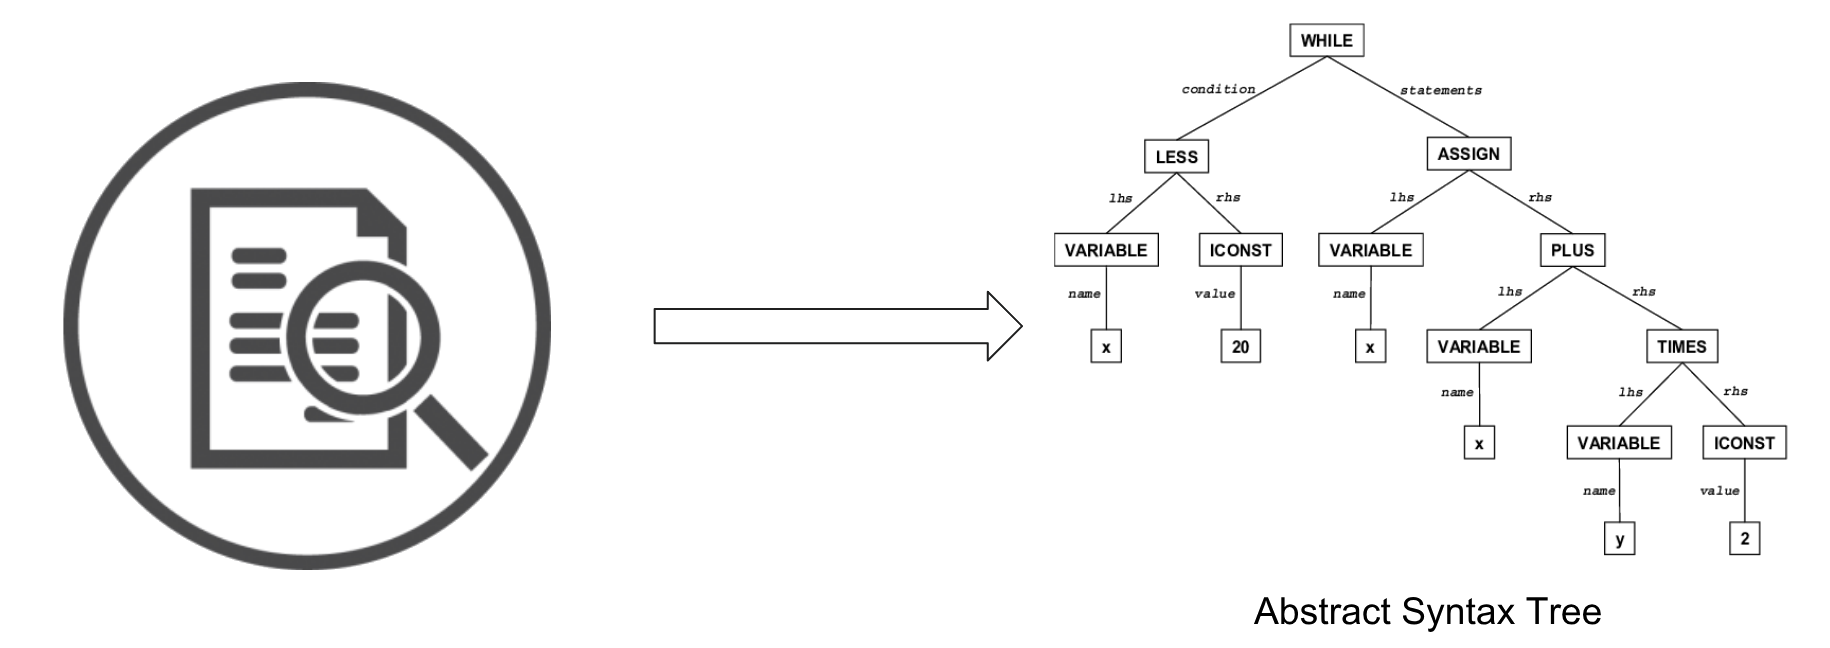
\includegraphics[width=1.0\textwidth]{images/ast.png}
	\end{center}
\end{frame}

\begin{frame}[fragile]{Analyzer Plugin}
		\begin{center}
      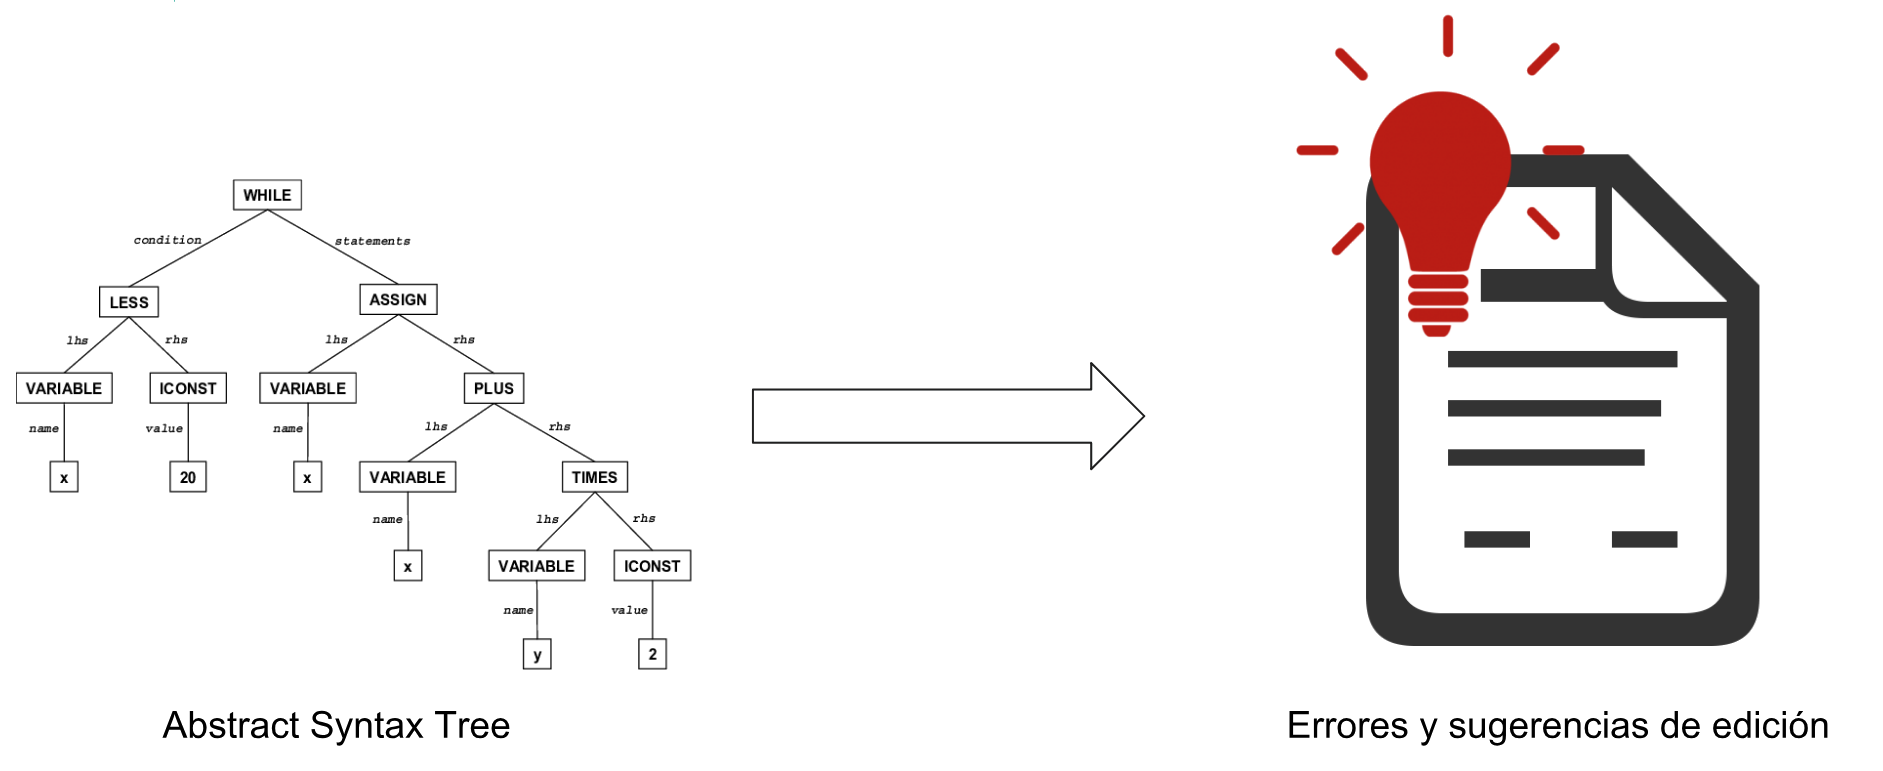
\includegraphics[width=1.0\textwidth]{images/plugin.png}
		\end{center}
\end{frame}

\begin{frame}[fragile]{Subconjunto soportado de Dart}
	\begin{center}
	\begin{lstlisting}[escapechar=!,basicstyle=\fontsize{9}{11}\ttfamily]
class Foo { !\pause!
  String foo(String a, String b) { !\pause!
    String s = "foo"; !\pause!
    if (a == b)!\pause! return a.concat(b);
    return s;
  }
}
  \end{lstlisting}
	\end{center}
\end{frame}

\begin{frame}[fragile]{Declaración de facetas públicas}
	Uso de anotaciones de Dart para declarar las facetas públicas. \\ \pause
	\vspace{1cm}
\begin{lstlisting}[escapechar=?,basicstyle=\fontsize{9}{9}\ttfamily]
bool login(String guess, @S("StringEq") String password) {
  return password.eq(guess);
}
\end{lstlisting}
\end{frame}

\begin{frame}[fragile]{Definición de facetas públicas}
	Uso de clases abstractas de Dart para declarar las facetas públicas. \\ \pause
	\vspace{1cm}
\begin{lstlisting}[escapechar=?,basicstyle=\fontsize{9}{9}\ttfamily]
bool login(String guess, @S("StringEq") String password) {
  return password.eq(guess);
}

abstract class StringEq {
  bool eq(String other);
}
\end{lstlisting}
\end{frame}
%
% \begin{frame}[fragile]{Pasos de la solución}
% 	\begin{enumerate}
% 		\item Definición del subconjunto de Dart soportado.
% 		\item Definición y declaración de facetas públicas en Dart.
% 		\alert{\item Integración de tipos estáticos comunes de Dart con las facetas de la desclasificación basada en tipos.}
% 		\item Definición de la gramática de tipos.
% 		\item Descripción del paso de generación de restricciones para un programa Dart.
% 		\item Descripción del paso de resolución de restricciones.
% 		\item Implementación de la extensión para ambientes de desarrollo.
% 	\end{enumerate}
% \end{frame}
%
% \begin{frame}[fragile]{Conversión de tipos de Dart a facetas privadas}
% 	\begin{onlyenv}<1>
% 		(código donde se usan tipos definidos por el usuario y tipos de dart)
% 	\end{onlyenv}
% 	\begin{onlyenv}<2>
% 		(código donde se usan tipos definidos por el usuario y tipos de dart, destacando tipo definido por el usuario)
% 	\end{onlyenv}
% 	\begin{onlyenv}<3>
% 		(código donde se usan tipos definidos por el usuario y tipos de dart, destacando tipo estático común de dart)
% 	\end{onlyenv}
% \end{frame}
%
% \begin{frame}[fragile]{Conversión de tipos de Dart a facetas privadas}
% 	\only<1->{(Mostrar operación de convert)}\\
% 	\only<2>{$P_{Bi}$ (algo)}
% 	\only<3>{$P_{Ai}$ (algo)}
%
% \end{frame}
%
% \begin{frame}[fragile]{Pasos de la solución}
% 	\begin{enumerate}
% 		\item Definición del subconjunto de Dart soportado.
% 		\item Definición y declaración de facetas públicas en Dart.
% 		\item Integración de tipos estáticos comunes de Dart con las facetas de la desclasificación basada en tipos.
% 		\alert{\item Definición de la gramática de tipos.}
% 		\item Descripción del paso de generación de restricciones para un programa Dart.
% 		\item Descripción del paso de resolución de restricciones.
% 		\item Implementación de la extensión para ambientes de desarrollo.
% 	\end{enumerate}
% \end{frame}
%
% \begin{frame}[fragile]{Gramática de tipos}
% 	\metroset{block=fill}
% 	\begin{block}{Gramática de tipos}
% 		\[\mathtt{\tau := \alpha\ |\ Obj(\overline{l: \tau})\ |\ \overline{\tau} \rightarrow \tau \ |\ \tau \sqcap \tau\ |\ \tau \sqcup \tau\ |\ Bot\ |\ Top}\]
% 	\end{block}
% \end{frame}
%
% \begin{frame}[fragile]{Pasos de la solución}
% 	\begin{enumerate}
% 		\item Definición del subconjunto de Dart soportado.
% 		\item Definición y declaración de facetas públicas en Dart.
% 		\item Integración de tipos estáticos comunes de Dart con las facetas de la desclasificación basada en tipos.
% 		\item Definición de la gramática de tipos.
% 		\alert{\item Descripción del paso de generación de restricciones para un programa Dart.}
% 		\item Descripción del paso de resolución de restricciones.
% 		\item Implementación de la extensión para ambientes de desarrollo.
% 	\end{enumerate}
% \end{frame}
%
% \begin{frame}[fragile]{Generación de restricciones}
% 	\begin{columns}[T,onlytextwidth]
% 		\column{0.6\textwidth}
% 		(Código con invocación a método y variables de tipo)
% 		\column{0.4\textwidth}
% 		(restricciones generadas)
% 	\end{columns}
% \end{frame}
%
% \begin{frame}[fragile]{Generación de restricciones}
% 	\begin{columns}[T,onlytextwidth]
% 		\column{0.6\textwidth}
% 		(Código con expresión de retorno y variables de tipo)
% 		\column{0.4\textwidth}
% 		(restricciones generadas)
% 	\end{columns}
% \end{frame}
%
% \begin{frame}[fragile]{Generación de restricciones}
% 	\begin{columns}[T,onlytextwidth]
% 		\column{0.6\textwidth}
% 		(Código con expresión de asignación y variables de tipo)
% 		\column{0.4\textwidth}
% 		(restricciones generadas)
% 	\end{columns}
% \end{frame}
%
% \begin{frame}[fragile]{Pasos de la solución}
% 	\begin{enumerate}
% 		\item Definición del subconjunto de Dart soportado.
% 		\item Definición y declaración de facetas públicas en Dart.
% 		\item Integración de tipos estáticos comunes de Dart con las facetas de la desclasificación basada en tipos.
% 		\item Definición de la gramática de tipos.
% 		\item Descripción del paso de generación de restricciones para un programa Dart.
% 		\alert{\item Descripción del paso de resolución de restricciones.}
% 		\item Implementación de la extensión para ambientes de desarrollo.
% 	\end{enumerate}
% \end{frame}
%
% \begin{frame}[fragile]{Resolución de restricciones}
% 	Simplificación de restricciones \\
% 	\only<2>{(Restricciones no simplificadas)}
% 	\only<3>{(Restricciones no simplificadas con obvias marcadas)}
% 	\only<4>{(Restricciones simplificadas)}
% \end{frame}
%
% \begin{frame}[fragile]{Resolución de restricciones}
% 	Agrupación de restricciones \\
% 	\only<1>{(Restricciones no agrupadas)}
% 	\only<2>{(Marcar con distinto color las restricciones de un grupo u otro)}
% 	\only<3>{(Restricciones agrupadas)}
% \end{frame}
%
% \begin{frame}[fragile]{Resolución de restricciones}
% 	Unificación: Construcción de tipos \\
% 	\only<1>{(Restricciones agrupadas)}
% 	\only<2>{(Restricciones agrupadas con candidatos a construcción marcados)}
% 	\only<3>{(Restricciones con nuevos tipos)}
% \end{frame}
%
% \begin{frame}[fragile]{Resolución de restricciones}
% 	Unificación: Verificación de restricciones \\
% 	\only<1>{(Restricciones)}
% 	\only<2>{(Restricciones con relaciones inválidas que provienen de invocación a método marcadas)}
% 	\only<3>{(Restricciones actualizadas luego de comprobación)}
% 	\only<4>{(Restricciones con relaciones inválidas que no provienen de invocación a método marcadas)}
% 	\only<5>{(Error generado por la restricción no válida)}
% \end{frame}
%
% \begin{frame}[fragile]{Resolución de restricciones}
% 	Unificación: Substitución de restricciones resueltas \\
% 	\only<1>{(Restricciones)}
% 	\only<2>{(Restricciones con restricciones resueltas marcadas)}
% 	\only<3>{(Substitución de restricciones)}
% \end{frame}
%
% \begin{frame}[fragile]{Resolución de restricciones}
% 	Unificación: Algoritmo iterativo \\
% 	\metroset{block=fill}
% 	\begin{block}{Algoritmo de unificación}
% 		(pseudocódigo del algoritmo)
% 	\end{block}
% \end{frame}
%
% \begin{frame}[fragile]{Pasos de la solución}
% 	\begin{enumerate}
% 		\item Definición del subconjunto de Dart soportado.
% 		\item Definición y declaración de facetas públicas en Dart.
% 		\item Integración de tipos estáticos comunes de Dart con las facetas de la desclasificación basada en tipos.
% 		\item Definición de la gramática de tipos.
% 		\item Descripción del paso de generación de restricciones para un programa Dart.
% 		\item Descripción del paso de resolución de restricciones.
% 		\alert{\item Implementación de la extensión para ambientes de desarrollo.}
% 	\end{enumerate}
% \end{frame}

\begin{frame}[fragile]{Extensión para ambientes de desarrollo}
	\begin{center}
		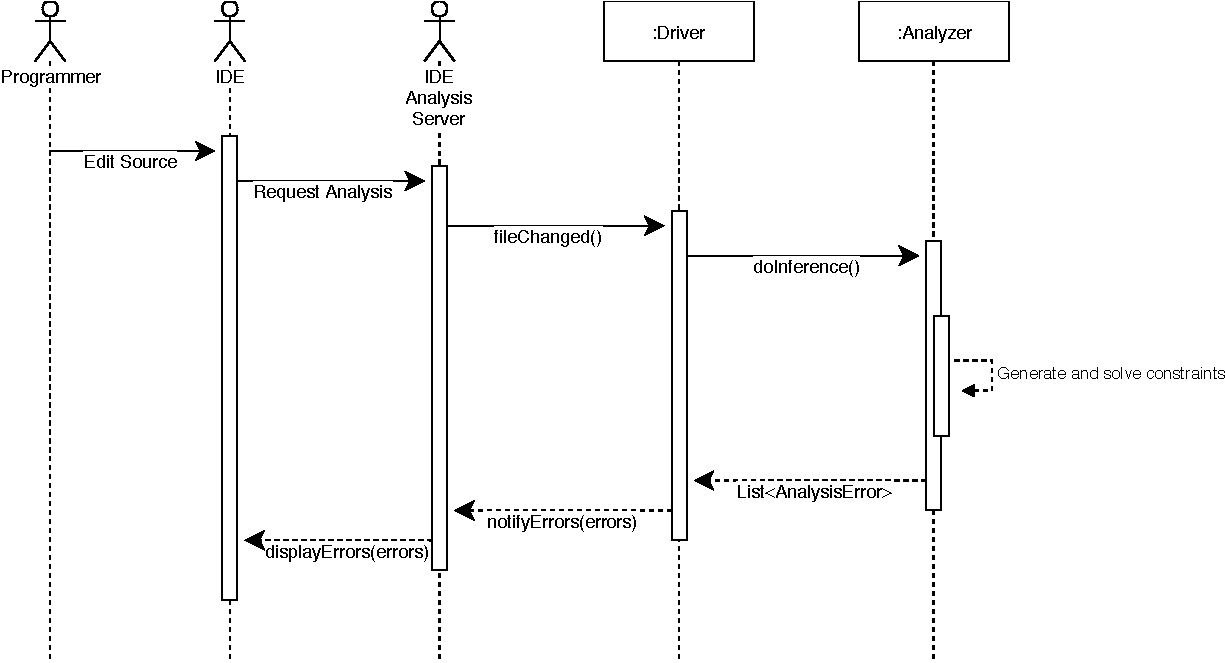
\includegraphics[width=0.8\textwidth]{images/sequence.pdf}
	\end{center}
\end{frame}

\begin{frame}[fragile]{Tipos de errores}
	Errores de seguridad \\ \pause
	\vspace{1cm}
\begin{lstlisting}[escapechar=?,basicstyle=\fontsize{9}{9}\ttfamily]
bool<bool login(String guess, @S("Top") String password) {
  ?\colorbox{red!20}{return password.eq(guess);}?
}
\end{lstlisting}
\end{frame}

\begin{frame}[fragile]{Tipos de errores}
	Errores de tipo mal formado \\ \pause
	\vspace{1cm}
\begin{lstlisting}[escapechar=?,basicstyle=\fontsize{9}{9}\ttfamily]
bool<Top login(String guess, ?\colorbox{red!20}{@S(\texttt{"}Abs") String password}?) {
  return password.eq(guess);
}

abstract class Abs {
  int abs();
}
\end{lstlisting}
\end{frame}

\begin{frame}[fragile]{Tipos de errores}
	Warning de faceta pública no definida \\ \pause
	\vspace{1cm}
\begin{lstlisting}[escapechar=?,basicstyle=\fontsize{9}{9}\ttfamily]
bool<bool login(String guess, ?\colorbox{yellow!50}{@S("StringEq")}? String password) {
  return password.eq(guess);
}
\end{lstlisting}
\end{frame}

\begin{frame}[fragile]{Tipos de errores}
	Información de faceta pública inferida \\ \pause
	\vspace{1cm}
\begin{lstlisting}[escapechar=?,basicstyle=\fontsize{9}{9}\ttfamily]
bool<bool login(String<String guess, String ?\underline{password}?) {
  return password.eq(guess);
} ?\pause?

password: [eq: String<String -> bool<bool]
\end{lstlisting}
\end{frame}

\section{Validación}

\begin{frame}[fragile]{Ejemplo: Sistema de autenticación web}
	\begin{center}
		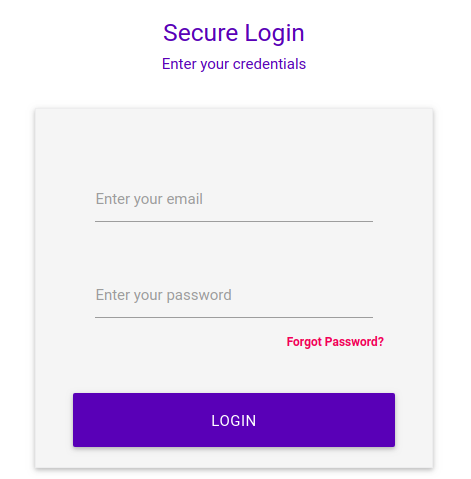
\includegraphics[width=0.5\textwidth]{images/screen4.png}
	\end{center}
\end{frame}

\begin{frame}[fragile]{Ejemplo: Sistema de autenticación web}
	\begin{center}
		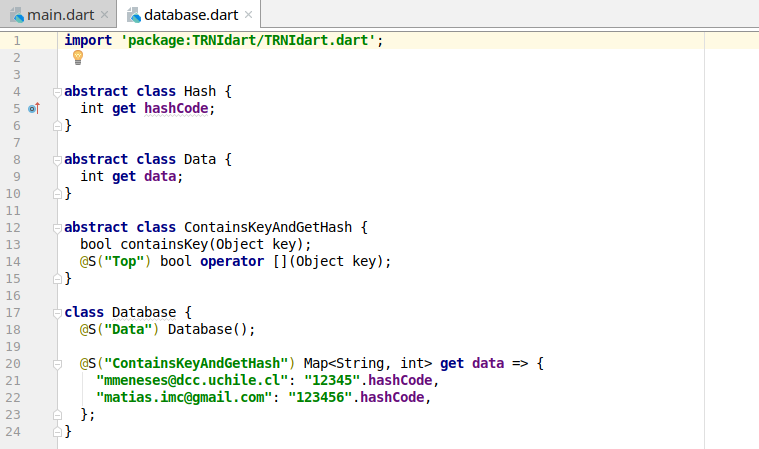
\includegraphics[width=0.95\textwidth]{images/database.png}
	\end{center}
\end{frame}

\begin{frame}[fragile]{Ejemplo: Sistema de autenticación web}
	\begin{center}
		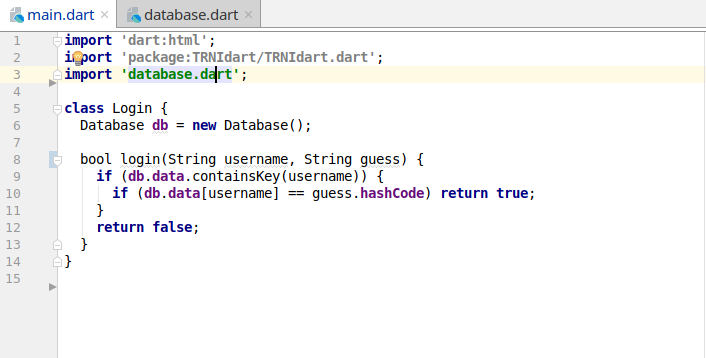
\includegraphics[width=1.0\textwidth]{images/login1.png}
	\end{center}
\end{frame}

\begin{frame}[fragile]{Ejemplo: Sistema de autenticación web}
	\begin{center}
		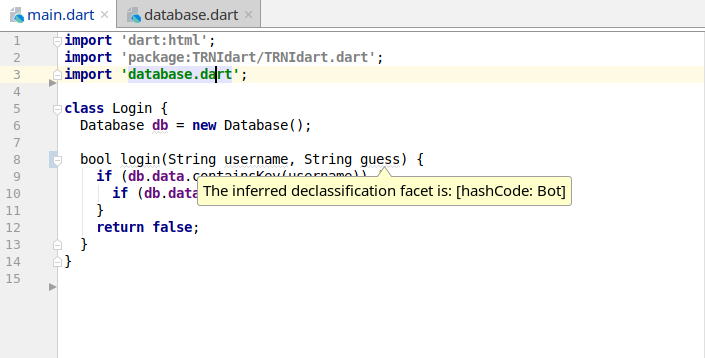
\includegraphics[width=1.0\textwidth]{images/login2.png}
	\end{center}
\end{frame}

\begin{frame}[fragile]{Ejemplo: Sistema de autenticación web}
	\begin{center}
		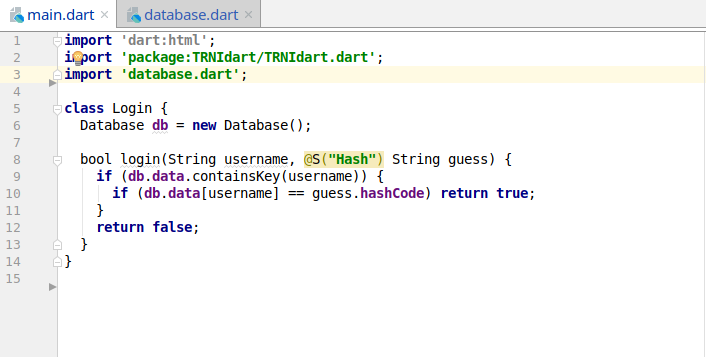
\includegraphics[width=1.0\textwidth]{images/login25.png}
	\end{center}
\end{frame}

\begin{frame}[fragile]{Ejemplo: Sistema de autenticación web}
	\begin{center}
		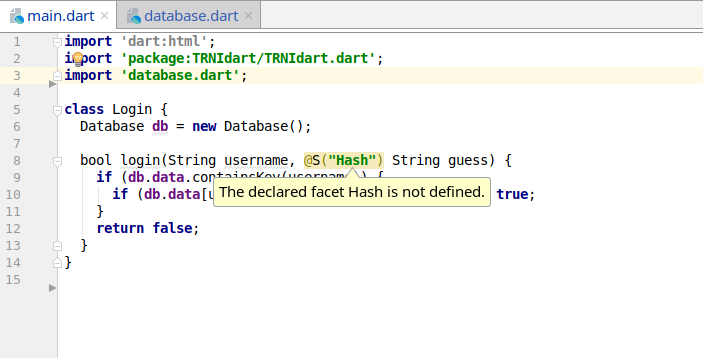
\includegraphics[width=1.0\textwidth]{images/login3.png}
	\end{center}
\end{frame}

\begin{frame}[fragile]{Ejemplo: Sistema de autenticación web}
	\begin{center}
		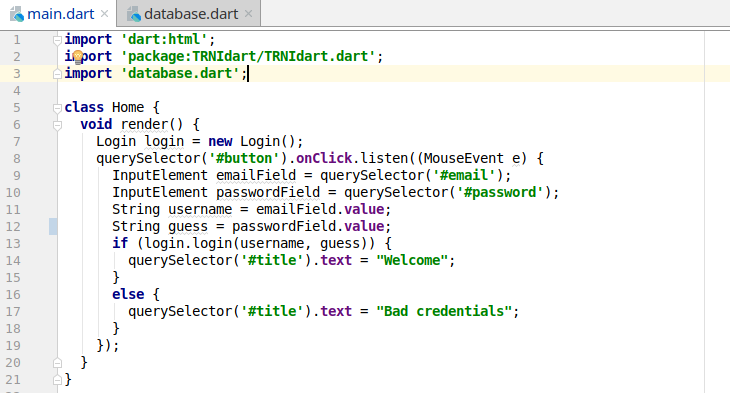
\includegraphics[width=1.0\textwidth]{images/html1.png}
	\end{center}
\end{frame}

\begin{frame}[fragile]{Ejemplo: Sistema de autenticación web}
	\begin{center}
		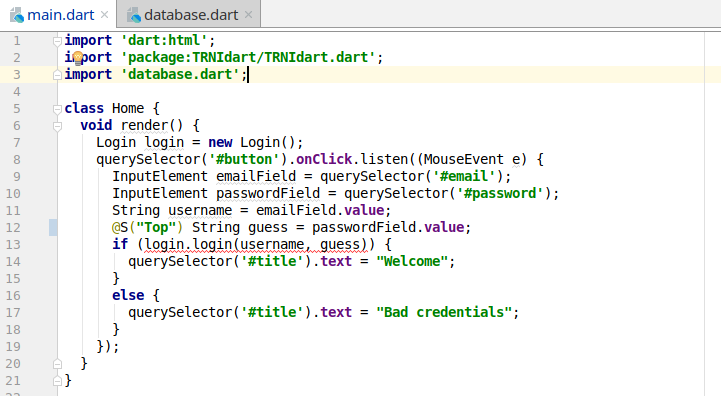
\includegraphics[width=1.0\textwidth]{images/html2.png}
	\end{center}
\end{frame}

\begin{frame}[fragile]{Ejemplo: Sistema de autenticación web}
	\begin{center}
		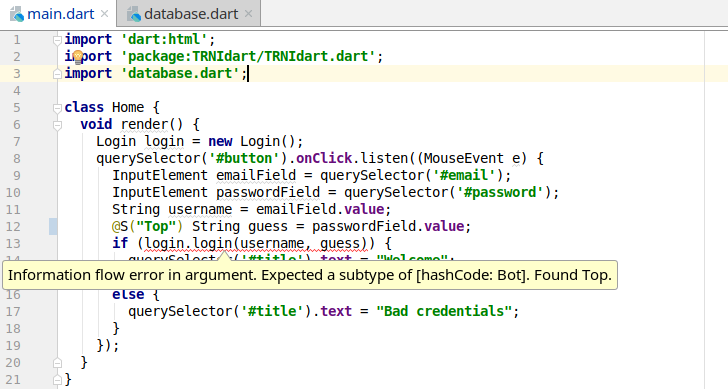
\includegraphics[width=1.0\textwidth]{images/html3.png}
	\end{center}
\end{frame}

\begin{frame}[fragile]{Ejemplo: Sistema de autenticación web}
	\begin{center}
		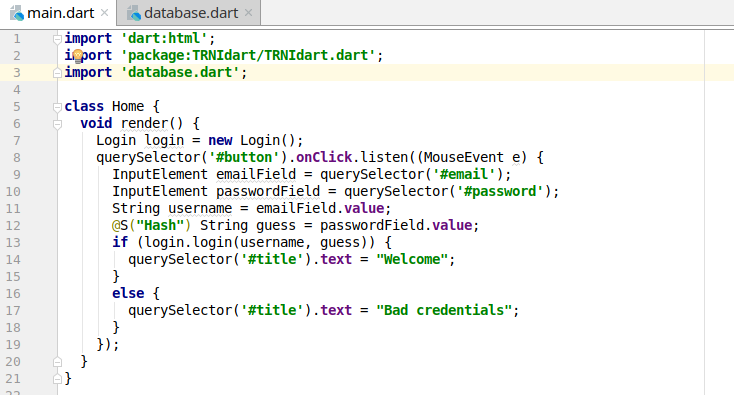
\includegraphics[width=1.0\textwidth]{images/html4.png}
	\end{center}
\end{frame}

\begin{frame}[fragile]{Ejemplo: Sistema de autenticación web}
	\begin{center}
		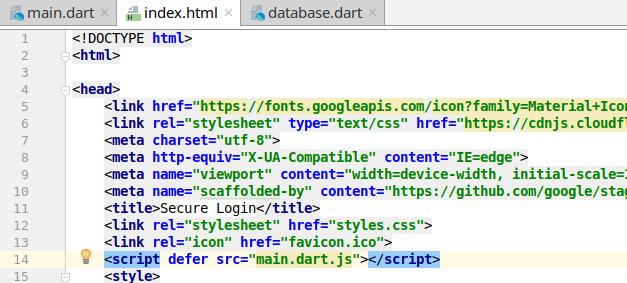
\includegraphics[width=1.0\textwidth]{images/html0.png}
	\end{center}
\end{frame}

\begin{frame}[fragile]{Ejemplo: Sistema de autenticación web}
	\begin{center}
		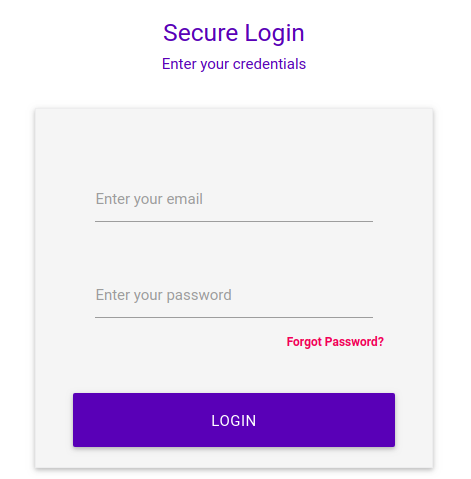
\includegraphics[width=0.5\textwidth]{images/screen4.png}
	\end{center}
\end{frame}

\begin{frame}[fragile]{Ejemplo: Sistema de autenticación web}
	\begin{table}
		\caption{Anotación de facetas públicas en identificadores}
		\begin{tabular}{c|c}
      Con inferencia & Sin inferencia\\
      \hline
      7 & 22\\
		\end{tabular}
	\end{table}
\end{frame}

\begin{frame}[fragile]{Comprobación de las reglas del sistema de tipos}
	Test unitarios en el repositorio del proyecto.
\end{frame}

\section{Conclusión}

\begin{frame}[fragile]{Conclusión}
	Conexión entre abstracciones de tipo y relaciones de orden de etiquetas de seguridad.
\end{frame}

\begin{frame}[fragile]{Trabajo futuro}
	Formalización de inferencia.
\end{frame}

\begin{frame}[fragile]{Trabajo futuro}
	Extensión al subconjunto soportado de Dart.
\end{frame}

\begin{frame}[fragile]{Trabajo futuro}
	Características de la extensión para ambientes de desarrollo.
\end{frame}

\begin{frame}[fragile]{Trabajo futuro}
	Extensión a polimorfismo. \\ \pause
	(lista parametrizada)
\end{frame}


{\setbeamercolor{palette primary}{fg=black, bg=yellow}
\begin{frame}[standout]
  Preguntas
\end{frame}
}

\appendix

\begin{frame}[fragile]{Apéndice}
  Cosas extra por posibles preguntas
\end{frame}


\end{document}
